\documentclass[a4paper]{article}
\usepackage[utf8]{inputenc}
\usepackage[czech]{babel}
\usepackage[margin=13mm, tmargin=15mm, bmargin=12mm]{geometry}
\usepackage{multirow}
\usepackage{tikz}
\usetikzlibrary{calc}
\usepackage{chngpage}
\usepackage{tabularx}
\usepackage{fancyhdr}
\usepackage{mathptmx}
\usepackage{lipsum}
\usepackage{float}
\usepackage{longtable}

\renewcommand{\baselinestretch}{1.15}
\pagenumbering{gobble}
\pagestyle{fancy}
\renewcommand{\headrulewidth}{0pt}

\newcommand{\jmeno}{David Škrob, Tomáš Názler, Radek Novotný}
\newcommand{\trida}{L4A}
\newcommand{\poradovecislo}{}
\newcommand{\nazevulohy}{PLC}
\newcommand{\cisloulohy}{}
\newcommand{\predmet}{Technické měření}
\newcommand{\skupina}{}
\newcommand{\datummereni}{19.1.2023}
\newcommand{\datumodevzdani}{}
\newcommand{\klasifikace}{}
\begin{document}
\fancyhead{
\begin{tikzpicture} [overlay,remember picture]
       \draw
        ($ (current page.north west) + (1cm, -12mm) $)
        rectangle
        ($ (current page.south east) + (-1cm,12mm) $);
\end{tikzpicture}
}

\renewcommand{\arraystretch}{2}
\shorthandoff{-}

{
\begin{adjustwidth}[]{-3mm}{-3mm}
\centering
\vspace*{-7mm}
\begin{tabularx}{\linewidth}{l|X|p{3cm}}
\multirow{2}{25mm}{\centering SPŠ a VOŠ technická Brno, Sokolská 1} &
\textbf{LABORATORNÍ CVIČENÍ Z ELEKTROTECHNIKY} & Třída: \trida \\
\cline{2-3}
 & Jméno a příjmení: \jmeno & Poř. Číslo: \poradovecislo \\
\hline
\end{tabularx}

\begin{tabularx}{\linewidth}{X|p{3cm}}
Název úlohy: \nazevulohy & Číslo úlohy: \cisloulohy \\
\hline
Zkoušený předmět: \predmet & Skupina: \skupina \\
\hline
\end{tabularx}

\begin{tabularx}{\linewidth}{X|X|X}
Datum měření: \datummereni &  Datum odevzdání: \datumodevzdani &  Klasifikace: \klasifikace \\
\hline
\end{tabularx}

\end{adjustwidth}
}

\shorthandon{-}


\section*{Zadání}
U každého úkolu nejprve sestavte pravdivostní tabulku, z ní napište rovnici
logické funkce, proved’te minimalizaci pomocí Karnaughovy mapy a naprogramujte do PLC. Protokol bude obsahovat všechny tyto kroky.
\begin{enumerate}
	\item Realizujte zapojení pro zadání Y5 z ”
	pracovního sešitu“ (text na
	fyzika.websy.cz, maturitní okruh č. 5).
	\item  Navrhněte logický obvod tak, aby signalizoval poplach tehdy, když
	ve výrobním procesu překročí dovolenou hodnotu alespoň 2 měřené
	veličiny ze 4 sledovaných.
	\item Navrhněte logický obvod hlasovacího zařízení pro čtyřčlennou komisi.
	Návrh projde, hlasuje-li pro návrh většina, při rovnosti hlasů rozhoduje
	hlas předsedy.
\end{enumerate}

\section*{Vypracování}
\begin{figure}[H]
	\centering
	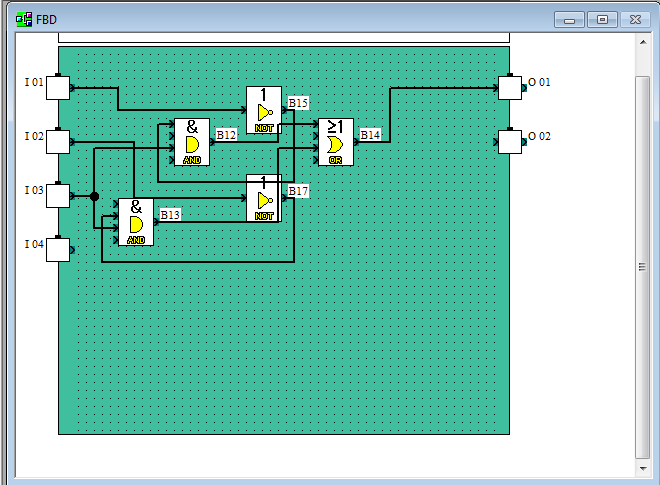
\includegraphics[width=0.7\textwidth]{PLC_1.png}
	\caption{Zapojení úkolu 1}
	\label{fig:mesh1}
\end{figure}

\begin{figure}[H]
	\centering
	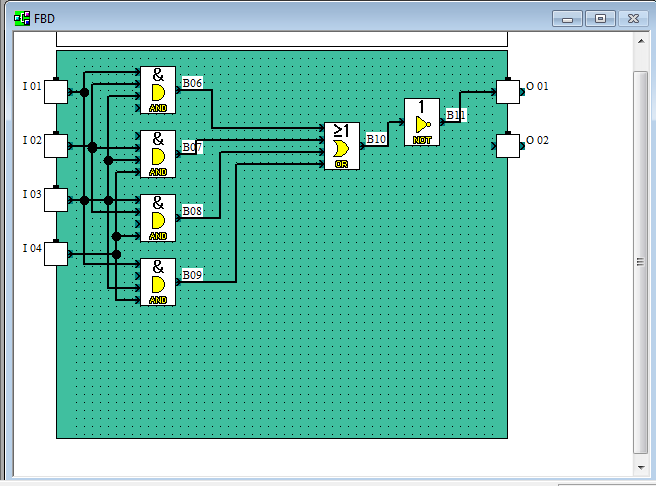
\includegraphics[width=0.7\textwidth]{PLC_2.png}
	\caption{Zapojení úkolu 2}
	\label{fig:mesh2}
\end{figure}

\begin{figure}[H]
	\centering
	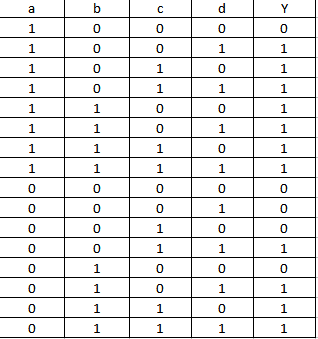
\includegraphics[width=0.3\textwidth]{hodnoty1.png}
	\caption{Seznam hodnot k úkolu 2}
	\label{fig:hodnoty1}
\end{figure}

\begin{figure}[H]
	\centering
	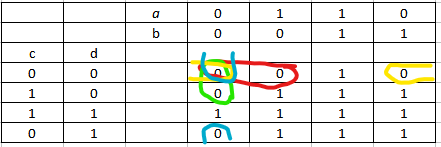
\includegraphics[width=0.3\textwidth]{hodnoty3.png}
	\caption{Karnaughova mapa k úkolu 2}
	\label{fig:hodnoty2}
\end{figure}


\begin{figure}[H]
	\centering
	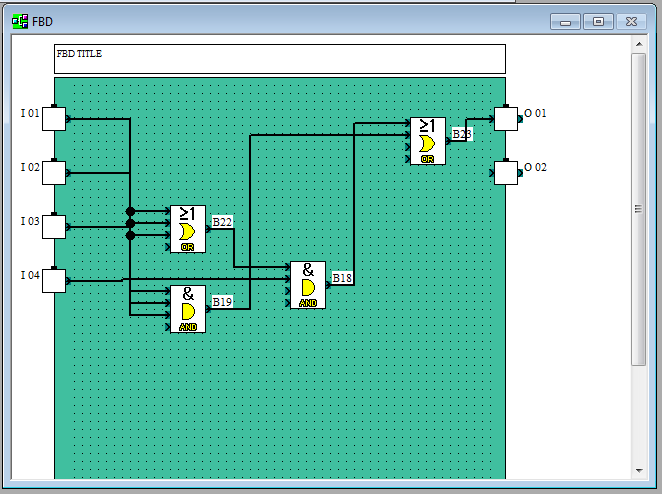
\includegraphics[width=0.7\textwidth]{PLC_3.png}
	\caption{Zapojení úkolu 3}
	\label{fig:mesh3}
\end{figure}

\begin{figure}[H]
	\centering
	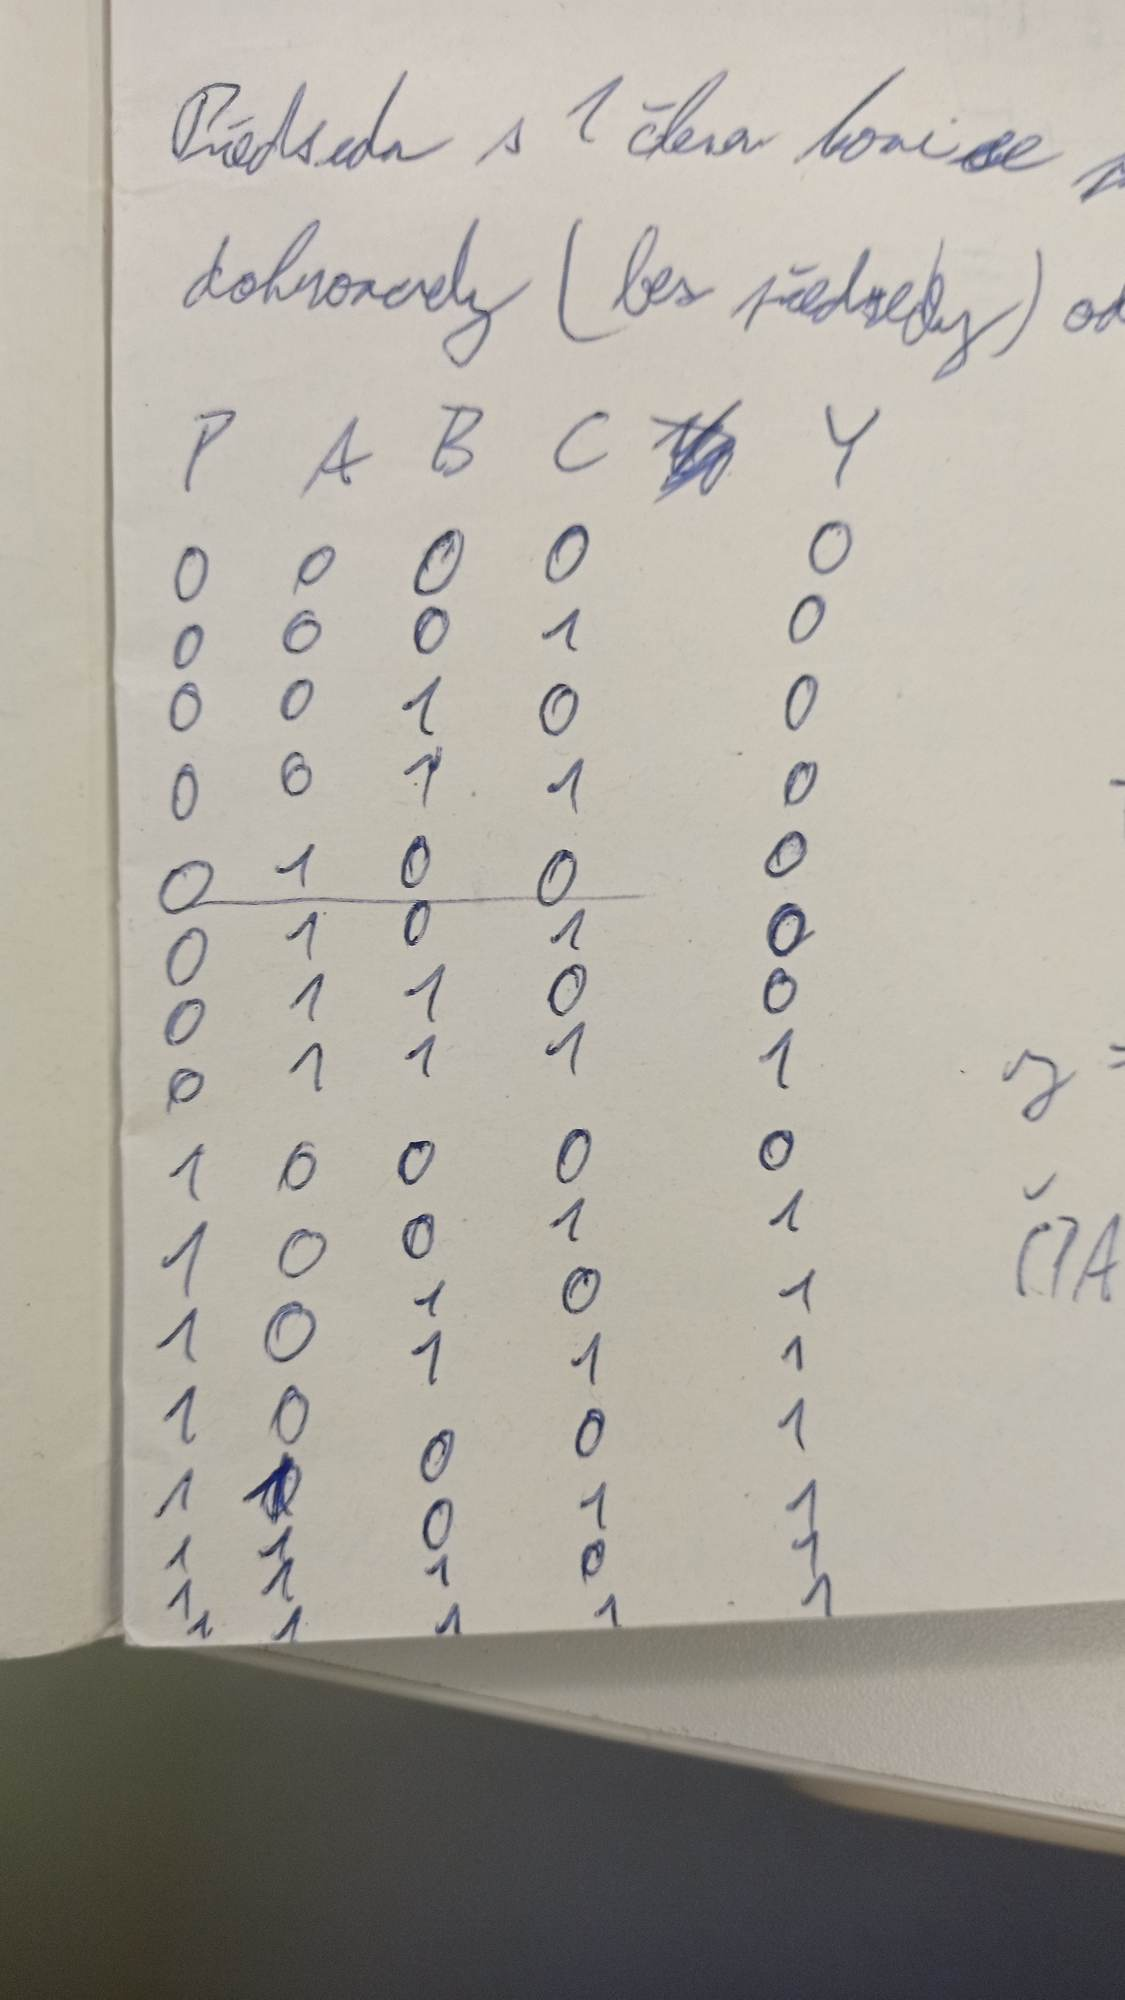
\includegraphics[width=0.3\textwidth]{foto1.jpg}
	\caption{Seznam hodnot k úkolu 3}
	\label{fig:foto1}
\end{figure}

\begin{figure}[H]
	\centering
	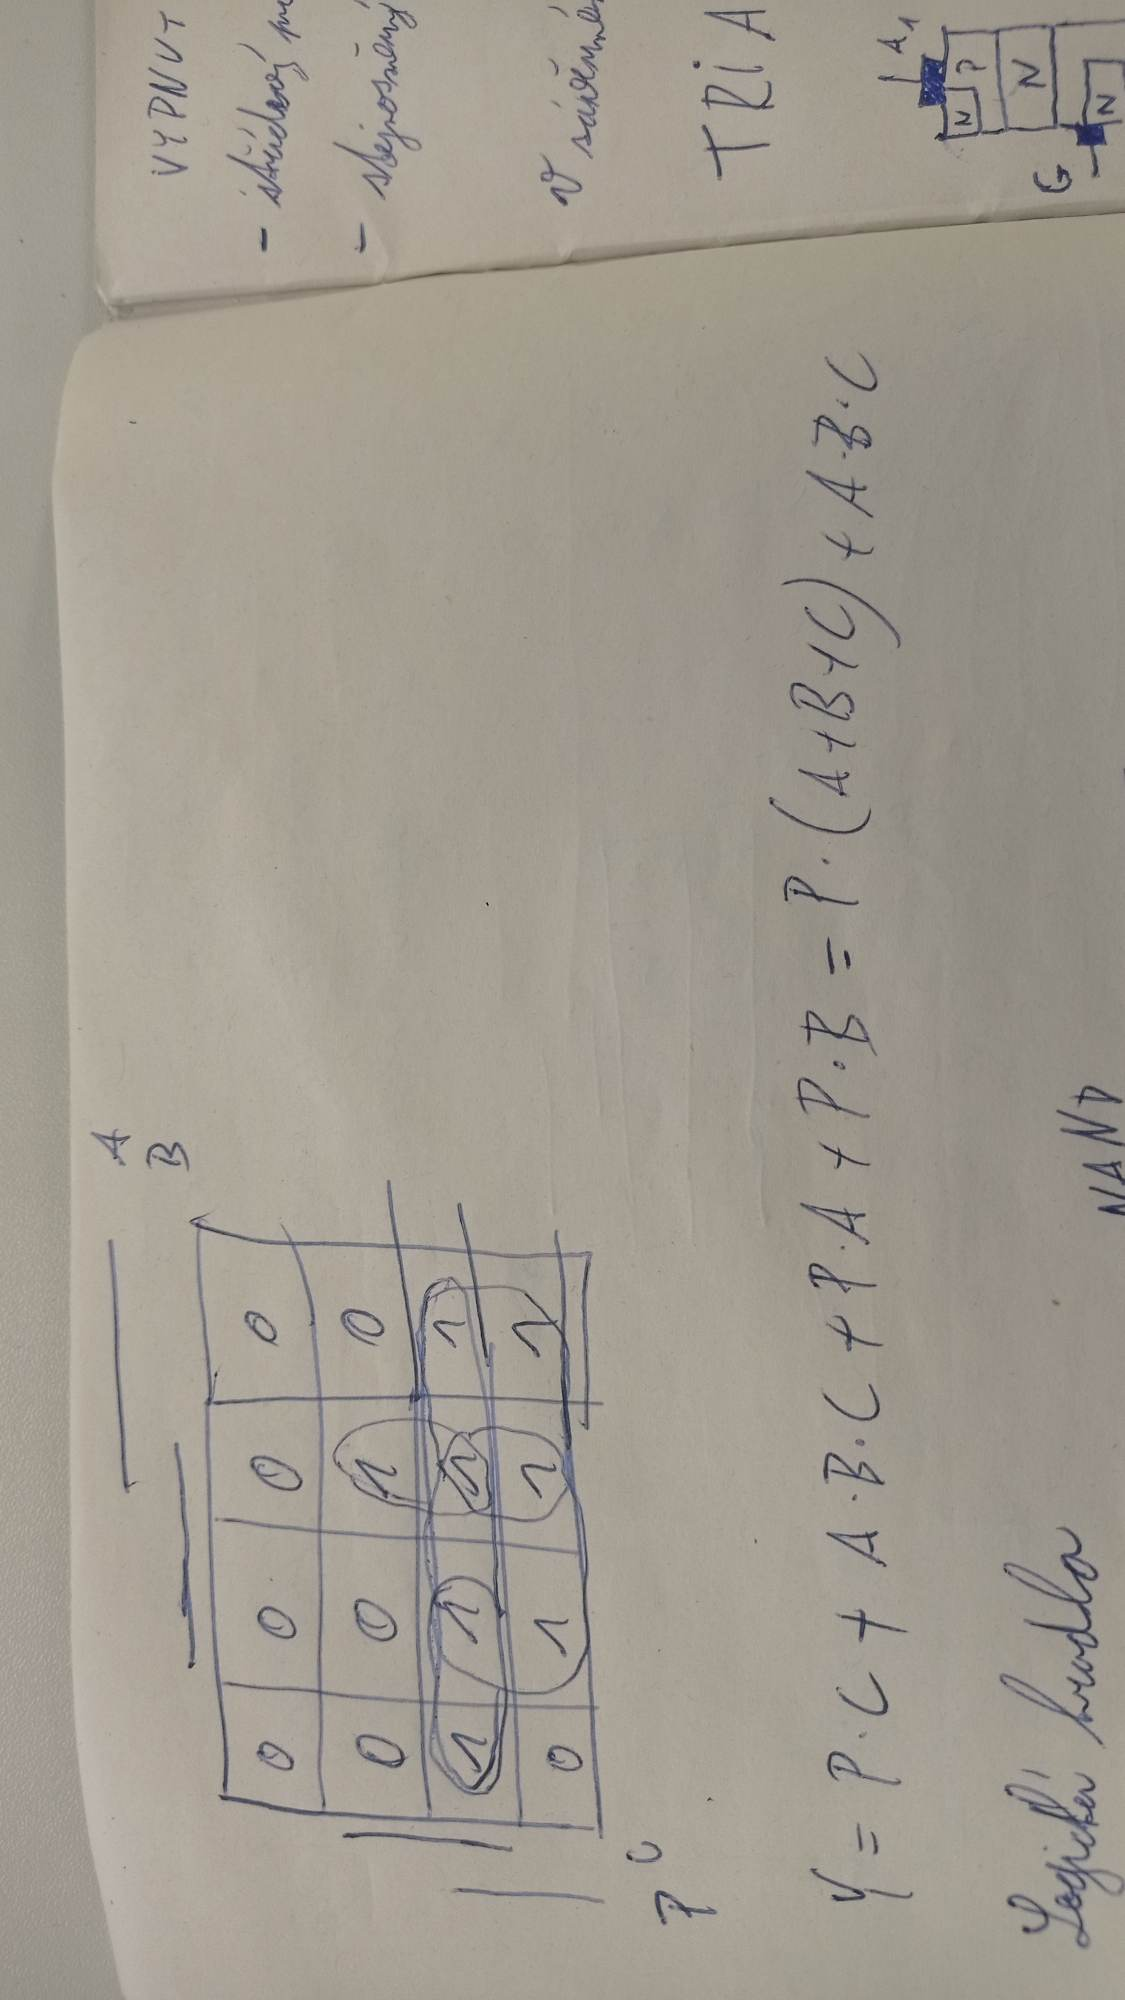
\includegraphics[width=0.3\textwidth, angle=270]{foto2.jpg}
	\caption{Karnaughova mapa k úkolu 3}
	\label{fig:foto2}
\end{figure}

\section*{Závěr}
Prace s softwerem \textit{Alpha} pro nás nebyla moc náročná, logické hradla umime jednoduše využit, tudíž zadané ulohy pro nás byly jednoduché. Protože máme kompletní poznámky v sešitě z minulého roku tak jsme našli již zhotovenou Karnaughova mapu pro zadaní úkolu čislo 3. Tudíž jsme zvládli práci na PLC v rekordním čase.
\vfill
\section*{Použité pomucky:}
\begin{tabularx}{\linewidth}{c|c|c|c}
	Přístroj – pomůcka & Typ & Rozsah (pouze analogové)
	& Poznámka \\
	\hline
	PLC & mas 6 rca & &
\end{tabularx}
\end{document}